\documentclass[border=10pt]{standalone}
\usepackage{tikz}
\usetikzlibrary{arrows.meta, positioning, calc, fit, backgrounds, decorations.pathreplacing}
\usepackage{xcolor}
\usepackage{amsmath}

% Brand colors
\definecolor{Garnet}{HTML}{73000A}
\definecolor{Atlantic}{HTML}{466A9F}
\definecolor{Congaree}{HTML}{1F414D}
\definecolor{Horseshoe}{HTML}{65780B}
\definecolor{Rose}{HTML}{CC2E40}
\definecolor{Honeycomb}{HTML}{A49137}
\definecolor{LightGray}{HTML}{ECECEC}
\definecolor{Black90}{HTML}{363636}
\definecolor{Black70}{HTML}{5C5C5C}
\definecolor{Black50}{HTML}{A2A2A2}
\definecolor{Black30}{HTML}{C7C7C7}
\definecolor{WarmGrey}{HTML}{676156}

\begin{document}
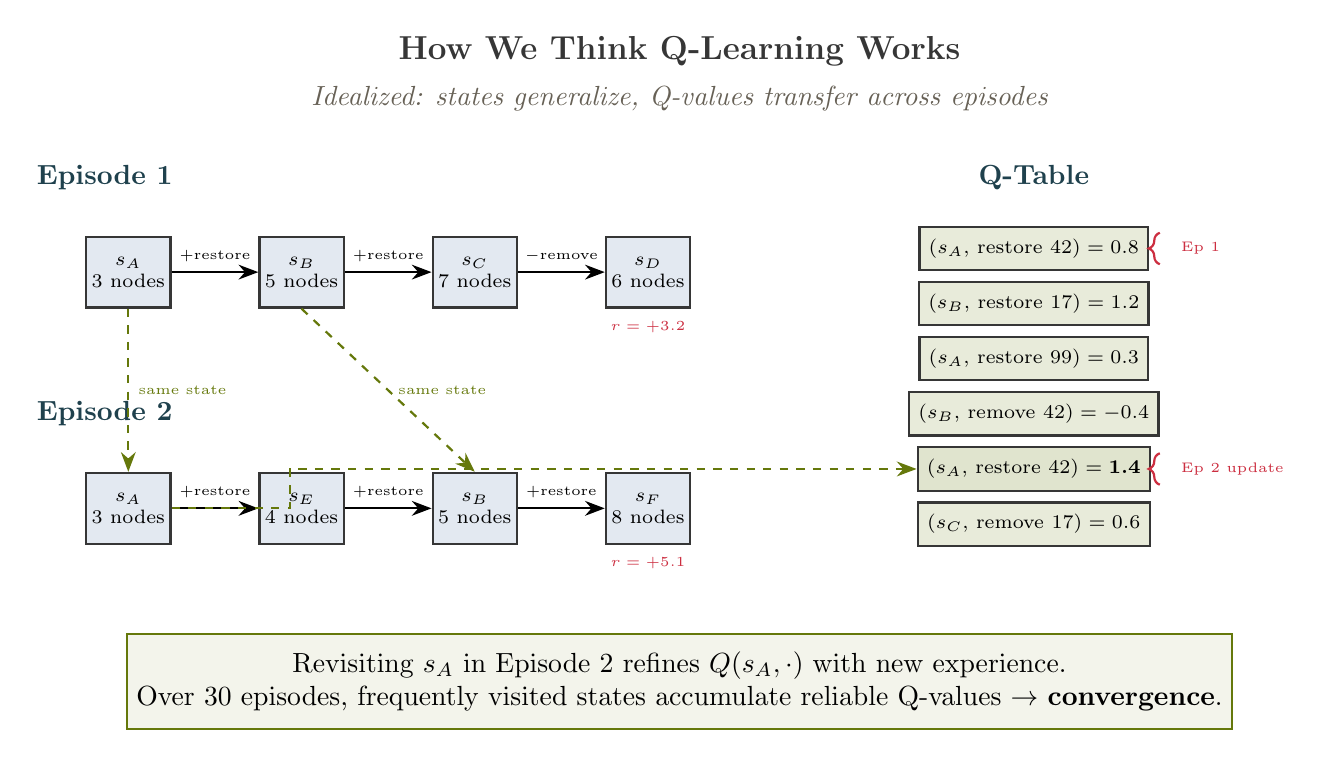
\begin{tikzpicture}[
    every node/.style={font=\small},
    state/.style={draw=Black90, thick, minimum size=0.9cm, inner sep=2pt,
        align=center, font=\scriptsize},
    qtable/.style={draw=Black90, thick, minimum width=2.6cm, minimum height=0.55cm,
        align=center, font=\scriptsize},
    arr/.style={-{Stealth[length=2.5mm]}, thick},
    eparr/.style={-{Stealth[length=2.5mm]}, thick, Horseshoe},
]

% === Title ===
\node[font=\large\bfseries, Black90] at (7.0, 8.8) {How We Think Q-Learning Works};
\node[font=\normalsize\itshape, WarmGrey] at (7.0, 8.2) {Idealized: states generalize, Q-values transfer across episodes};

% =============================================
% EPISODE 1
% =============================================
\node[font=\normalsize\bfseries, Congaree] at (-0.3, 7.2) {Episode 1};

\node[state, fill=Atlantic!15] (e1s1) at (0, 6.0) {$s_A$\\3 nodes};
\node[state, fill=Atlantic!15] (e1s2) at (2.2, 6.0) {$s_B$\\5 nodes};
\node[state, fill=Atlantic!15] (e1s3) at (4.4, 6.0) {$s_C$\\7 nodes};
\node[state, fill=Atlantic!15] (e1s4) at (6.6, 6.0) {$s_D$\\6 nodes};

\draw[arr] (e1s1) -- (e1s2) node[midway, above, font=\tiny] {+restore};
\draw[arr] (e1s2) -- (e1s3) node[midway, above, font=\tiny] {+restore};
\draw[arr] (e1s3) -- (e1s4) node[midway, above, font=\tiny] {$-$remove};

\node[font=\tiny, Rose] at (6.6, 5.3) {$r = +3.2$};

% =============================================
% EPISODE 2
% =============================================
\node[font=\normalsize\bfseries, Congaree] at (-0.3, 4.2) {Episode 2};

\node[state, fill=Atlantic!15] (e2s1) at (0, 3.0) {$s_A$\\3 nodes};
\node[state, fill=Atlantic!15] (e2s2) at (2.2, 3.0) {$s_E$\\4 nodes};
\node[state, fill=Atlantic!15] (e2s3) at (4.4, 3.0) {$s_B$\\5 nodes};
\node[state, fill=Atlantic!15] (e2s4) at (6.6, 3.0) {$s_F$\\8 nodes};

\draw[arr] (e2s1) -- (e2s2) node[midway, above, font=\tiny] {+restore};
\draw[arr] (e2s2) -- (e2s3) node[midway, above, font=\tiny] {+restore};
\draw[arr] (e2s3) -- (e2s4) node[midway, above, font=\tiny] {+restore};

\node[font=\tiny, Rose] at (6.6, 2.3) {$r = +5.1$};

% =============================================
% SHARED STATE ARROWS (the ideal)
% =============================================
% s_A in ep1 matches s_A in ep2
\draw[eparr, dashed] (e1s1.south) -- (e2s1.north)
    node[midway, right, font=\tiny, text=Horseshoe] {same state};

% s_B in ep1 matches s_B in ep2
\draw[eparr, dashed] (e1s2.south) -- (e2s3.north)
    node[midway, right, font=\tiny, text=Horseshoe] {same state};

% =============================================
% Q-TABLE (shows meaningful accumulation)
% =============================================
\node[font=\normalsize\bfseries, Congaree] at (11.5, 7.2) {Q-Table};

\node[qtable, fill=Horseshoe!15] (q1) at (11.5, 6.3)
    {$(s_A$, restore 42$) = 0.8$};
\node[qtable, fill=Horseshoe!15] (q2) at (11.5, 5.6)
    {$(s_B$, restore 17$) = 1.2$};
\node[qtable, fill=Horseshoe!15] (q3) at (11.5, 4.9)
    {$(s_A$, restore 99$) = 0.3$};
\node[qtable, fill=Horseshoe!15] (q4) at (11.5, 4.2)
    {$(s_B$, remove 42$) = -0.4$};
\node[qtable, fill=Horseshoe!20] (q5) at (11.5, 3.5)
    {$(s_A$, restore 42$) = \textbf{1.4}$};
\node[qtable, fill=Horseshoe!15] (q6) at (11.5, 2.8)
    {$(s_C$, remove 17$) = 0.6$};

% Arrow from shared states to Q-table
\draw[arr, Horseshoe, dashed] (e2s1.east) -- ++(1.5, 0) |- (q5.west);

% Annotation: value updated
\draw[decorate, decoration={brace, amplitude=4pt, mirror}, thick, Rose]
    (13.1, 6.5) -- (13.1, 6.1) node[midway, right=4pt, font=\tiny, text=Rose] {Ep 1};
\draw[decorate, decoration={brace, amplitude=4pt, mirror}, thick, Rose]
    (13.1, 3.7) -- (13.1, 3.3) node[midway, right=4pt, font=\tiny, text=Rose] {Ep 2 update};

% =============================================
% BOTTOM: convergence narrative
% =============================================
\node[draw=Horseshoe, thick, fill=Horseshoe!8, minimum width=13.5cm,
    minimum height=1.2cm, align=center, font=\normalsize] at (7.0, 0.8)
    {Revisiting $s_A$ in Episode 2 refines $Q(s_A, \cdot)$ with new experience.\\
    Over 30 episodes, frequently visited states accumulate reliable Q-values $\rightarrow$ \textbf{convergence}.};

\end{tikzpicture}
\end{document}
